\section{Symmetric Monoidal Bicategories}
\label{sec:constr-symm-mono}

In this section we will discuss how the iconic functor $\mathcal{H}$ from section~\ref{sec:1x1-to-bicat} extends to a functor of locally cubical bicategories. Furthermore, we will show that it preserves the monoidal structure functorially. We will do this by proving that the functor preserves products, and that every product preserving functor defines a functor between the respective locally cubical bicategories of monoidal cells. 

%Note that there are several related notions of these locally cubical bicategories, depending on whether we want the functors to be lax monoidal, oplax monoidal, or strongly monoidal. We will discuss the lax case in this section. In the next section we will generalise this result. 
%t was shown in~\cite{gg:ldstr-tricat} that tricategories, lax homomorphisms, ico-icons and pseudo-icons form a locally cubical bicategory. As a monoidal bicategory is a tricategory with one object, it follows that monoidal bicategories, lax monoidal functors, lax icons and lax transformations form a locally cubical bicategory as well. 
Double categories, pseudo double functors and tight transformations form a locally cubical bicategory with identity tight 2-morphisms and identity 3-cells. The functor $\comp$ is defined on tight transformations as the Godement product. The pseudo functor $\compI_A: * \rightarrow \cD bl(A,A)$ maps the cells in the trivial double category $*$ to the identity cells and morphisms in $\cD bl(A,A)$. 

As described in~\cite{gg:ldstr-tricat}, bicategories, pseudo functors, pseudo transformations, icons and cubical modifications also form a locally cubical bicategory. We will recall the definition of icons and cubical modifications and describe the enriched structure of this category.

\begin{anfxnote}[author=MS]{icons}
  What context is this definition in?
  Is it just the usual notion  of icon between functors of bicategories?
  If so, why are $\D$ and $\E$ written in double-category font and some of the arrows are marked with the ``loose'' bullet?
\end{anfxnote}

\begin{defn}
Let $F,G: \D \rightarrow \E$ be pseudo functors. an {\bf icon} $\alpha: F \Rightarrow G$ is given by a family of 2-cells $\alpha_f : Ff \Rightarrow Gf$ indexed by the 1-cells of $\D$, which are natural in $f$ and such that for all objects $A, B, C$ and 1-cells $A \xrightarrow{f} B \xrightarrow{g} C$ the following diagrams commute:
\[
\begin{tikzpicture}[xscale=1.5]
\node (tl) at (0,1) {$\id_{FA}$};
\node (tr) at (1,1) {$F \id_A$};
\node (bl) at (0,0) {$\id_{GA}$};
\node (br) at (1,0) {$G\id_A$};
\draw[doubleloose] (tl) to node[above]{$\iso$} (tr);
\draw[doubleloose] (bl) to node[below]{$\iso$} (br);
\draw[doubleeq] (tl) to (bl);
\draw[doubletight] (tr) to node[right]{$\alpha_{\id_A}$} (br);
\end{tikzpicture}\qquad
\begin{tikzpicture}[xscale=2]
\node (tl) at (0,1) {$Fg  Ff$};
\node (tr) at (1,1) {$F(gf)$};
\node (bl) at (0,0) {$Gg Gf$};
\node (br) at (1,0) {$G(gf)$};
\draw[doubleloose] (tl) to node[above]{$\iso$} (tr);
\draw[doubleloose] (bl) to node[below]{$\iso$} (br);
\draw[doubletight] (tl) to node[left]{$\alpha_g \alpha_f$}(bl);
\draw[doubletight] (tr) to node[right]{$\alpha_{gf}$} (br);
\end{tikzpicture}
\]
\end{defn}
% By globular tight transformations, we  mean tight transformations $\alpha: F \rightarrow G$ between two functors that agree on objects, such that the family $\{\alpha_f\}$ consists of globular 2-cells. A cubical double modification is defined analogously to a cubical modification~\cite{gg:ldstr-tricat}.

\begin{defn}
Let $F,G,H,K: \D \rightarrow \E$ be pseudo functors; let $\alpha: F \looseRightarrow G$, $\beta: H \looseRightarrow K$ be pseudo transformations; let $\gamma: F \looseRightarrow H$, $\delta: G \looseRightarrow K$ be icons. A cubical modification
\[
\begin{tikzpicture}
\node (tl) at (0,1) {$F$};
\node (tr) at (1,1) {$G$};
\node (bl) at (0,0) {$H$};
\node (br) at (1,0) {$K$};
\draw[doubleloose] (tl) to node[above]{$\alpha$} (tr);
\draw[doubleloose] (bl) to node[below]{$\beta$} (br);
\draw[doubletight] (tl) to node[left]{$\gamma$} (bl);
\draw[doubletight] (tr) to node[right]{$\delta$} (br);
\node at (.5,.5) {$\DDownarrow \Gamma$};
\end{tikzpicture}
\]
is given by a family of 2-cells $\Gamma_A: \alpha_A \RRightarrow \beta_A$ such that for every 1-cell $f:A \rightarrow B$ of $\D$, the following equality holds.

 \begin{equation}
 \begin{aligned}
 \begin{tikzpicture}[scale=1.5]
 \node (tl) at (-1,1) {$FA$};
 \node (tm) at (0,1) {$FB$};
 \node (tr) at (1,1) {$GB$};
 \node (bl) at (-1,0) {$FA$};
 \node (bm) at (0,0) {$GA$};
 \node (br) at (01,0) {$GB$};
 \node (bl1) at (-1,-.7){$HA$};  
 \node (bm1) at (0,-.7) {$KA$};
 \node (br1) at (1,-.7) {$KB$}; 
 \draw[doubleloose] (tm)  to node[above]{$\alpha_B$} (tr);
 \draw[doubleeq] (bm) to (bm1);
 \draw[doubleloose] (bm) to node[above] {$Gf$}(br);
 \draw[doubleeq] (tr) to (br);
 \draw[doubleeq] (tl)  to  (tm);
 \draw[doubleeq] (tl) to (bl);
 \draw[doubleloose] (tl) to node[above]{$Ff$}(tm);
 \draw[doubleloose] (bl) to node[above]{$\alpha_A$}(bm);
 \node at (0,.5) {\footnotesize $\Downarrow \alpha_f$}; 
 \node at (0.5,-.3) {\footnotesize $\Downarrow \delta_f$}; 
  \node at (-0.5,-.3) {\footnotesize $\Downarrow \Gamma_A$};
 \draw[doubleloose] (bl1)  to node[above]{$\beta_A$} (bm1);
 \draw[doubleloose] (bm1) to  node[above]{$Kf$}(br1);
 \draw[doubleeq] (bl)  to (bl1);
 \draw[doubleeq] (br)  to (br1);
 \end{tikzpicture}
 \end{aligned}
 =
\begin{aligned}
 \begin{tikzpicture}[scale=1.5]
 \node (tl) at (-1,1) {$FA$};
 \node (tm) at (0,1) {$FB$};
 \node (tr) at (1,1) {$GB$};
 \node (bl) at (-1,0) {$HA$};
 \node (bm) at (0,0) {$HB$};
 \node (br) at (01,0) {$KB$};
 \node (bl1) at (-1,-.7){$HA$};  
 \node (bm1) at (0,-.7) {$KA$};
 \node (br1) at (1,-.7) {$KB$}; 
 \draw[doubleloose] (tm)  to node[above]{$\alpha_B$} (tr);
 \draw[doubleeq] (tm) to (bm);
 \draw[doubleloose] (bm) to node[above] {$\beta_B$}(br);
 \draw[doubleeq] (tr) to (br);
 \draw[doubleeq] (tl)  to  (tm);
 \draw[doubleeq] (tl) to (bl);
 \draw[doubleloose] (tl) to node[above]{$Ff$}(tm);
 \draw[doubleloose] (bl) to node[above]{$Hf$}(bm);
 \node at (-0.5,.5) {\footnotesize $\Downarrow \gamma_f$}; 
 \node at (0.5,.5) {\footnotesize $\Downarrow \Gamma_B$}; 
 \draw[doubleloose] (bl1)  to node[above]{$\beta_A$} (bm1);
 \draw[doubleloose] (bm1) to  node[above]{$Kf$}(br1);
 \draw[doubleeq] (bl)  to (bl1);
 \draw[doubleeq] (br)  to (br1);
 \node at (0,-0.3) {\footnotesize $\DDownarrow \beta_f$}; 
 \end{tikzpicture}
 \end{aligned}
\end{equation}

\end{defn}

The pseudo functor $\compI_A: * \rightarrow \cB icat(A,A)$ maps the cells in the trivial bicategory $*$ to the identity cells and morphisms of $\cB icat(A,A)$. 
The pseudofunctor $\comp$ is defined on functors as composition in the iconic tricategory $\cB icat$. On pseudo transformations and icons it is given by the Godement product. On cubical modifications it is defined below:

\begin{equation*}
\begin{aligned}
 \begin{tikzpicture}[scale=2]
 \node (tl) at (-1,1) {$FF'A$};
 \node (tm) at (0,1) {$GF'A$};
 \node (tr) at (1,1) {$GG'A$};
 \node (bl) at (-1,0) {$HF'A$};
 \node (bm) at (0,0) {$KF'A$};
 \node (br) at (01,0) {$KG'A$};
 \node (bl1) at (-1,-1){$HH'A$};  
 \node (bm1) at (0,-1) {$KH'A$};
 \node (br1) at (1,-1) {$KK'A$}; 
 \draw[doubleloose] (tm)  to node[above]{$G(\alpha'_A)$} (tr);
 \draw[doubleeq] (tm) to (bm);
 \draw[doubleloose] (bm) to node[above] {$K(\alpha'_A)$}(br);
 \draw[doubleeq] (tr) to (br);
 \draw[doubleeq] (tl)  to  (tm);
 \draw[doubleeq] (tl) to (bl);
  \draw[doubleeq] (bm) to (bm1);
 \draw[doubleloose] (tl) to node[above]{$\alpha_{F'A}$}(tm);
 \draw[doubleloose] (bl) to node[above]{$\beta_{F'A}$}(bm);
 \node at (-0.5,.5) {\footnotesize $\Downarrow \Gamma_{F'A}$}; 
 \node at (0.5,.5) {\footnotesize $\Downarrow \delta_{\alpha'_A}$}; 
 \draw[doubleloose] (bl1)  to node[above]{$\beta_{H'A}$} (bm1);
 \draw[doubleloose] (bm1) to  node[above]{$K(\beta'A)$}(br1);
 \draw[doubleeq] (bl)  to (bl1);
 \draw[doubleeq] (br)  to (br1);
 \node at (-.5,-0.5) {\footnotesize $=$}; 
\node at (.5,-0.5) {\footnotesize $\DDownarrow K\Gamma'_A$}; 
\end{tikzpicture}
\end{aligned}
\end{equation*}
%%%%%%%%%

Functoriality follows from naturality of the icons. Note that there are several canonical ways to define this composition on cubical modifications, by choosing different versions of the Godement product.  

\fxnote[author=MS]{See earlier comment about this condition.}
For $\cB icat$ and $\cD bl$, all identity cells are lax monoidal. In fact, all identity cells are strong monoidal braided, sylleptic and symmetric. This means that the requirements from the previous section is satisfied; hence, the locally cubical bicategories $\cMon \cDbl$ and $\cMon \cBicat$ of monoidal cells and morphisms of $\cDbl$ and $\cBicat$, respectively, are well-defined.

We upgrade the functor from theorem 4.11 to a functor of locally cubical bicategories.


\begin{defn}\label{def:lcbcfunc}
Let ${\bf S,T}$ be locally cubical bicategories. A functor $\cT: {\bf T} \rightarrow {\bf S}$ consists of the following data:
\begin{enumerate}
\item An assignment on objects that sends each object $A$ of ${\bf T}$ to an object $\cT A$ of ${\bf S}$.
\item For each two objects $A,B$, a pseudo double functor (1-cell in \cDbl) ${\bf T}(A,B) \rightarrow {\bf S}(\cT(A),\cT(B))$
\item For every triple of objects $A,B,C$ of ${\bf T}$, a tight transformation (2-cell in $\cD bl$) 
\begin{align} 
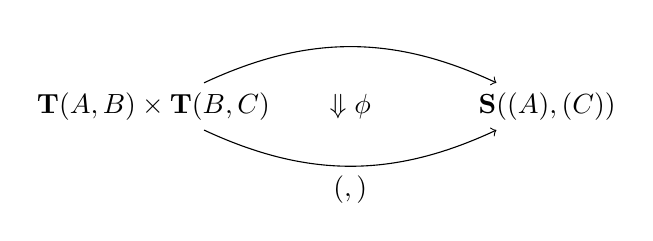
\begin{tikzpicture}
\node(1) at (0,0) {${\bf T}(A,B) \times {\bf T}(B,C)$};
\node(2) at (5,0) {${\bf S}(\cT(A),\cT(C))$};
\draw[->] (1) to[in=155, out=25] node[above]{$\cT \comp $} (2); 
\draw[->] (1) to[in=-155, out=-25] node[below]{$ \comp (\cT,\cT)$} (2); 
\node at (2.5,0) {$\Downarrow \phi \iso$};
\end{tikzpicture}
\end{align}
\item For every object $A$ of {\bf T} a tight transformation
\begin{align}
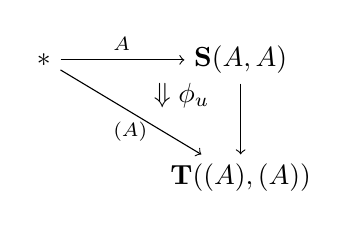
\begin{tikzpicture}[xscale=.5, yscale=.3]
\node(1) at (0,0) {$*$};
\node(2) at (5,0) {${\bf S}(A,A)$};
\node(3) at (5,-5) {${\bf T}(\cT(A),\cT(A))$};
\draw[->] (1) to node[above]{$\looseid_{A}$} (2); 
\draw[->] (1) to node[below]{$\looseid_{\cT(A)}$} (3);
\draw[->] (2) to node[right]{$\cT$} (3); 
\node at (3.5,-1.5) {$\Downarrow \phi_u \iso$};
\end{tikzpicture}
\end{align}
\item The usual coherence diagrams, Definition 10 of~\cite{nick:tricatsbook} commute.
\end{enumerate}
\end{defn}



\begin{prop}
The iconic functor $\cH: \cD bl_{\bf f} \rightarrow \cB icat$ extends to a functor of locally cubical bicategories $\fH: \fDbl_{\bf f} \rightarrow \fBicat$ that preserves products.
\end{prop}

\begin{proof}
For any $\D, \E$, the double category $\fDblf(\D, \E)$ has only globular 2-cells and is identical to the bicategory in section~\ref{sec:1x1-to-bicat}. Consequently, each pseudo functor $\cH: \cDbl(\D,\E) \rightarrow \cBicat(\cH\D, \cH \E)$ corresponds to a pseudo double functor $\fH: \fDblf(\D,\E) \rightarrow \fBicat(\fH\D, \fH \E)$. The icons $\phi$ and $\phi_u$ then define tight transformations consisting of globular 2-cells and the coherence diagrams are automatically satisfied. The proof that $\cH$ preserves product carries directly over to the case of $\fH$.
\end{proof}


 \begin{lem}\label{lem:funcmonob}
  Let ${\bf S,T}$ be locally cubical bicategories with products. Let $\mathcal{T}: T \rightarrow S$ be a functor such that the tight transformations $\phi$, $\phi_u$ are globular. If $F$ preserves products, it preserves  monoidal objects, 1-cells, 2-cells, icons and 3-cells as well as any braided, sylleptic or symmetric structure on the objects, 1-cells,2-cells, icons and 3-cells.
 \end{lem}
 
 \begin{proof}
Let $A$ be a monoidal object. As the functor $\mathcal{T}$ preserves products, we have a product $\cT(A) \times_{\cT} \cT(A) = \cT(A \times A)$. As a consequence $\ten\maps
  A\times A\to A$ induces 1-cells $\ten_{\mathcal{T}} \maps
 \mathcal{T}A\times_{\cT} \mathcal{T} A\to\mathcal{T}A$ and $I_{\cT}:= \mathcal{T}(I_A)$. 
 
Since $\phi$ and $\phi_u$ are globular, we have an equality $\cT(f \comp g) = \cT(f) \comp \cT(g)$ for all $f$ and $g$ and for the identity 1-cell we have an equality $\cT(\transid_A) = \transid_{\cT(A)}$. The loose associativity 2-cell of $A$ gives rise to a loose 2-cell
  \[\vcenter{\xymatrix@C=6pc{\cT(A)\times\cT(A)\times\cT(A) \rtwocell^{\ten_{\cT}
        (\Id\times\ten_{\cT})}_{\ten_{\cT}(\ten_{\cT}\times\Id)}{\hspace{.2cm}\fa_{\cT}\eqv} &\cT(A) }}\]
  which simply equals $\cT(\alpha)$ together with the invertible 2-cells.
  
  Likewise, the unit constraints $l, r$ as well as the constraints for (braided) monoidal 1-cells $\sigma$ induce 1-cells $l_{\cT}, r_{\cT}$, and $\sigma_{\cT}$, respectively. Note that the swap functor $\tau$ is mapped by $\cT$ to the swap functor for the product $\times_{\cT}$, so $\sigma_{\cT}$ is well-defined.
  
 Furthermore, the invertible 3-cell filling the Mac Lane pentagon lifts to the invertible 3-cell of the Mac Lane Pentagon for $\cT(A)$. Which is simply its image under $\cT$, composed the natural transformations $\cT_{\odot}$, $\phi$,and $\phi_u$ ensuring that it has the right type.
%   \[\xy
%  (-10,0)*{\ten_{\cT}(\ten_{\cT},\Id)(\ten_{\cT}, \Id, %\Id)}="A";
%  (20,10)*{\ten_{\cT}(\ten_{\cT},\Id)(\Id, \ten_{\cT},\Id)}="B";
%  (50,0)*{\ten_{\cT}(\Id,\ten_{\cT})(\Id, \ten_{\cT},\Id)}="C";
%  (0,-15)*{\ten_{\cT}(\Id, \ten_{\cT})(\ten, \Id, \Id)}="D";
%  (40,-15)*{\ten_{\cT}(\Id, \ten_{\cT})(\Id, \Id, \ten, _{\cT})}="E";
%  (20,-5)*{\scriptstyle\Downarrow \pi \iso};
%  \ar "B";"A";^{\fa_{\cT} \ten_{\cT} \id}
%  \ar "C";"B";^{\fa_{\cT}}
%  \ar "D";"A";_{\fa_{\cT}}
%  \ar "E";"D";_{\fa_{\cT}}
%  \ar "E";"C";^{\id\ten_{\cT} \fa_{\cT}}
%  \endxy
%  \]
  
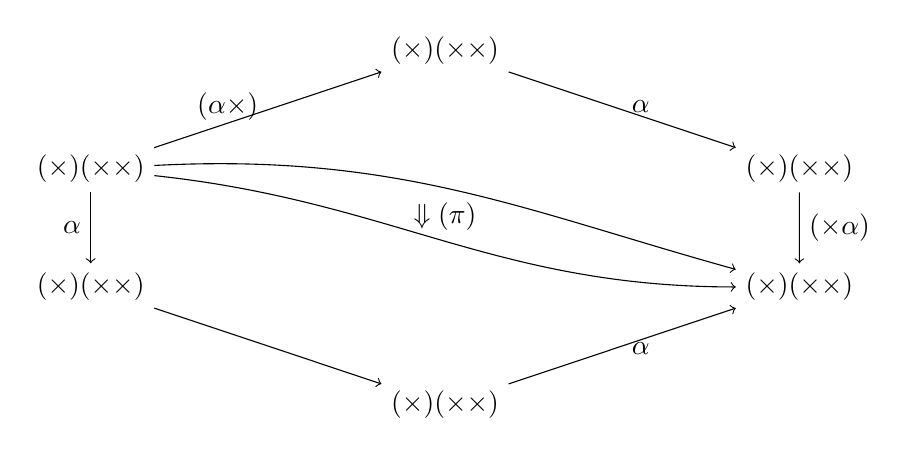
\begin{tikzpicture}[yscale=1.5, xscale=3]
\node(tl) at (0,1) {$\ten (\ten \times \transid)(\ten \times \transid \times \transid)$};
\node(t) at (1.5,2) {$\ten (\ten \times \transid)(\transid \times \ten \times \transid)$};
\node(tr) at (3,1) {$\ten (\transid \times \ten )(\transid \times \ten \times \transid)$};
\node(br) at (3,0) {$\ten (\transid \times \ten )(\transid \times \transid \times \ten )$};
\node(b) at (1.5,-1) {$\ten (\ten \times \transid)(\transid \times \transid \times \ten )$};
\node(bl) at (0,0) {$\ten (\transid \times \ten )(\ten \times \transid \times \transid)$};
\draw[->] (tl) to node[left, yshift=1pt] {$\looseid (\alpha \times \looseid)$} (t);
\draw[->] (t) to node[right, yshift=1pt] {$\alpha \looseid$} (tr);
\draw[->] (tr) to node[right] {$\looseid (\looseid \times \alpha)$} (br);
\draw[->] (tl) to node[left] {$\alpha \looseid$} (bl);
\draw[->] (bl) to node[left,yshift=-1pt] {$\looseid$} (b);
\draw[->] (b) to node[right,yshift=-1pt] {$\alpha \looseid$} (br);
\draw[->] (tl) to [in=155, out=5] (br);
\draw[->] (tl) to [in=180, out=-10] (br);
%\draw[->] (tl) to [in=180, out=10](tr);
%\draw[->] (bl) to [in=185, out=0](br);
\node at (1.5,.6) {$\Downarrow \cT(\pi) \iso$};
%\node at (2.5,.6) {$\Downarrow \phi^{-1} \iso$};
%\node at (1.5,1.5) {$\Downarrow \phi^{-1} \iso$};
%\node at (.5,.4) {$\Downarrow \phi \iso$};
%\node at (1.5,-.5) {$\Downarrow \phi \iso $};
\node at (2,1) {$\iso$};
\node at (1,0) {$\iso $};
\end{tikzpicture}  

 Note that there may be several way to past these 3-cells, but by coherence of enriched pseudo functors, the result is the same. Likewise, the isomorphic 3-cells $\mu, \lambda,\rho$ and the isomorphic 3-cells $R,S$, and $v$ witnessing the braiding and syllepsis, lift to the appropriate 3-cell for $\cT(A)$. This is also the case for the isomorphic 3-cells $R,S$ that characterise the braiding. 
   Finally,  the three equations between pasting composites of $\pi_{\cT}, \mu_{\cT}, \lambda_{\cT}, \rho_{\cT}$ hold by coherence of enriched pseudo functors.

%Similarly, we prove that $\cT$ preserves braided, sylleptic and symmetric structure. The swap functor $\tau$ is mapped by $\cT$ to the swap functor for the product $\times_{\cT}$. It follows that the braiding 2-cell $\sigma: \tens \looseRightarrow \tens \tau$  gives rise to a braiding 

%\[\vcenter{\xymatrix@C=6pc{\cT(A)\times\cT(A) \rtwocell^{\ten_{\cT}
  %      }_{\ten_{\cT}\tau}{\hspace{.2cm}\sigma_{\cT}\eqv} &\cT(A) }}\]
        
%Analogously to $\alpha$, the invertible globular 3-cells $S, T$, and $\upsilon$ are lifted to their images under $\cT$, augmented with instances of $\phi$ to ensure that the 3-cells have the right type. 

Similarly, one can show that for a monoidal transformation $f$, $\cT(f)$ is monoidal with structure loose 2-cells $\cT(\iota_f)$ and $\cT(\chi_f)$ and 3-cells obtained from $\cT(\omega),  \cT(\gamma)$, and $\cT(\delta)$ analogously to $\alpha$. If $f$ is braided, the braiding of $\cT(f)$ is witnessed by the 3-cell obtained from $\cT(u)$. Likewise, $\cT$ preserves any monoidal, braided, sylleptic and symmetric structure of tight 2-morphisms, loose 2-cells and 3-cells. 
 \end{proof}


\begin{thm}\label{thm:lcbcfunctor}
Let $F: \cC  \rightarrow \cD$ be a functor of locally cubical bicategories, such that the tight transformations $\phi$, $\phi_u$ are globular. If $F$ preserves products, then it lifts to the functors below between locally cubical bicategories, for $w \in \{l,o,s\}$.
\begin{align*}
&\cM on_wF: \cM on_w \cC  \rightarrow \cM on_w\cD\\ 
&\cBr \cM on_wF: \cBr \cM on_w \cC  \rightarrow \cBr \cM on_w\cD\\
& \cSyl \cM on_wF: \cSyl \cM on_w \cC  \rightarrow \cSyl \cM on_w\cD\\
&\cSym \cM on_wF: \cSym \cM on_w \cC  \rightarrow \cSym \cM on_w\cD
\end{align*}
\end{thm}

\begin{proof}
By Lemma~\ref{lem:funcmonob}, the assignment of $F$ on objects and higher cells is well-defined in the respective categories.
We wil show that functor $F$ gives rise to a pseudo double functor $\cM on_lF: \cM on_l \cC(A, B)  \rightarrow \cM on_l\cD(\cM on_lF(A), \cM on_lF(B))$. The other functors are derived in a similar way. We need to verify that $F(N^{\alpha \verc \beta}) = F(N^{\alpha}) \verc F(N^{\beta})$ and $F(N^{\tightid_f}) = N^{\tightid_{Ff}}$ in $\cM on_l\cD$ and likewise for $\Sigma$. This follows from functoriality of $F$, the fact that $N^{\alpha \verc \beta} = N^{\alpha \verc \beta}$ and $N^{\tightid_f} = \tightid_{\iota_f}$, $F(\iota_f) = \iota_{Ff}$.
The natural transformations $F_{\odot}$ and $F_U$ are well-defined 3-cells in $\cM onD$; the respective equations hold by coherence of the pseudo double functor $F$.
Finally, we need to prove that $\phi$ and $\phi_u$ are well-defined tight transformations in $\cM on(\cT A, \cT B)$. Since their components are globular 3-cells, we only need to check that these are monoidal. The equations hold by coherence of enriched functors after expanding the definitions of $M^{\cT\alpha \comp \cT \beta}, M^{\cT(\alpha \comp \beta)}, M^{\cT(\looseid_f)}$, and $M^{\looseid_{\cT f}}$ and similarly for $\Pi$.
\end{proof}

Note that in the case of $\cH$, $\phi$ and $\phi_u$ have globular components. It follows that the functor $\fH: \fDbl_f \rightarrow \fBicat$ lifts to the functors $\cM on_w \fH: \cMon_w\fDbl_f \rightarrow \cMon_w \fBicat$, $\cBr_w \fH: \cBr_w\fDbl_f \rightarrow \cBr_w \fBicat$,  $\cSyl_w\cH: \cSyl_w\fDbl_f \rightarrow \cSyl_w\fBicat$, and $\cSym_w \fH: \cSym_w\fDbl_f \rightarrow \cSym_w \fBicat$.
\fxnote{Let's state a precise ``theorem'' here as a conclusion.}


% Local Variables:
% TeX-master: "smbicat"
% End:
